\begin{figure*}[!ht]
    \centering
    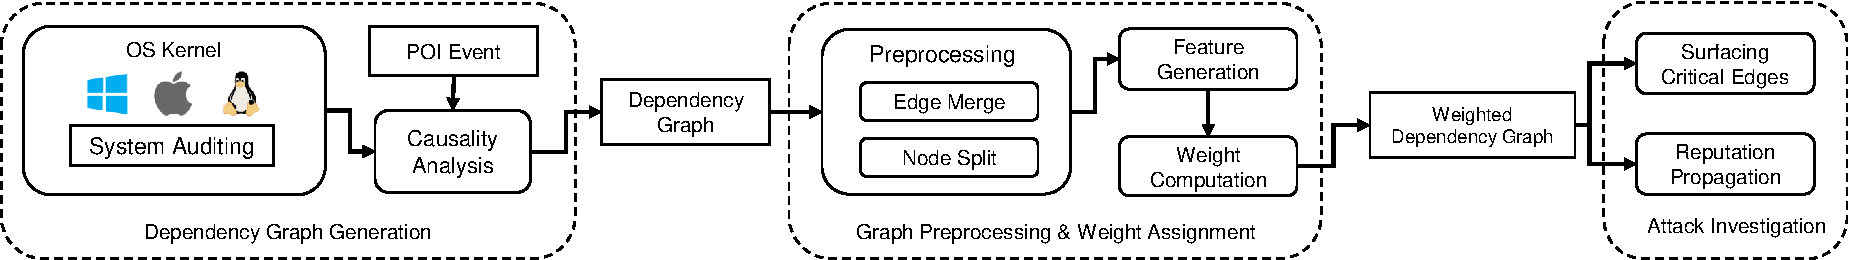
\includegraphics[width=0.95\textwidth,clip]{figs/overview-crop.pdf}
    \caption{Workflow of \tool}
    \label{fig:overview}
    \vspace*{-1ex}
\end{figure*}


\section{Overview and Threat Model}
\label{sec:overview}

\cref{fig:overview} shows the work flow of \tool. 
\tool consists of three phases: (1) dependency graph generation, (2) graph preprocessing \& weight assignment, and (3) attack investigation.
In the first phase, 
\tool leverages system auditing tools such as Auditd~\cite{auditd}, ETW~\cite{etw}, DTrace~\cite{dtrace}, and Sysdig~\cite{sysdig} to collect system level auditing events about system calls.
Given a POI event, \tool parses the collected events and applies causality analysis~\cite{backtracking,backtracking2} to obtain the dependency graph for the event.
In the second phase, 
  \tool performs graph preprocessing to merge the same type of edges between two nodes
and split the nodes to remove parallel edges between nodes.
This process transforms the dependency graph into a simple directed graph that is easier for weight computation and reputation propagation.
\tool then generates three types of features and computes the weights for each edge,
producing a weighted dependency graph.
In the third phase,
\tool surfaces critical edges by providing a suggested range of threshold values to prune non-critical edges,
and propagates reputations to identify malicious payloads.

\eat{
The main steps of the proposed framework can be summarized as follows: (i) System auditing tools are deployed on the host. (ii) System call activities are collected by the auditing tools and stored. (iii) A dependency graph is built out of the monitoring data and causality analysis is applied to reconstruct the time line of a given vertex of security significance. (iv) The graph is trimmed by merging redundant edges. (v) Vertices are split if there exists parallel edges. (vi) After these prepossessing steps, the weight of each edge in the graph is computed. (vii) Based on the weights, the reputation value of the system entity of interest in the graph is inferred by reputation propagation. (viii) Non-critical edges can be further pruned to achieve better human readability of the graph. Figure~\ref{fig:after} shows a sample dependency graph after the whole process of \tool. }



\myparatight{Threat Model}
\tool is a causality analysis tool over system monitoring data,
and thus we follow the threat model of previous works on system monitoring data~\cite{backtracking,backtracking2,loggc,trustkernel,gao2018aiql,gao2018saql,timelytrack}. 
We assume that the system monitoring data collected from kernel space~\cite{auditd,etw} is not tampered, and that the kernel is trusted.
Any kernel-level attack that deliberately compromises security auditing systems is beyond the scope of this work.

The attacker executes APT attacks involving multiple steps such as target discovery and data exfiltration. We assume an outside attacker that attacks the system remotely (from outside of the system). Thus, the attacker either utilizes the vulnerabilities in the system or convinces the user to download a file. The main goal of the attacker is to inject her malicious files into the victim’s system without being detected. In this work, we assume the attacker does not know how the proposed reputation system operates, and hence we do not consider the potential attacks against the reputation system. 

% We do consider that insiders or external attackers have full knowledge of the deployed \tool queries and the anomaly models. 
% They can launch attacks with seemingly ``normal'' activities to evade \dsl's anomaly detection,
% and may hide their attacks by mimicking peer hosts' behaviors to avoid \dsl's outlier detection.